%%%%%%%%%%%%%%%%%%%%%%%%%%%%%%%%%%%%%%%%%
% Beamer Presentation
% LaTeX Template
% Version 1.0 (10/11/12)
%
% This template has been downloaded from:
% http://www.LaTeXTemplates.com
%
% License:
% CC BY-NC-SA 3.0 (http://creativecommons.org/licenses/by-nc-sa/3.0/)
%
%%%%%%%%%%%%%%%%%%%%%%%%%%%%%%%%%%%%%%%%%

%----------------------------------------------------------------------------------------
%	PACKAGES AND THEMES
%----------------------------------------------------------------------------------------

\documentclass{beamer}

\mode<presentation> {

% The Beamer class comes with a number of default slide themes
% which change the colors and layouts of slides. Below this is a list
% of all the themes, uncomment each in turn to see what they look like.

%\usetheme{default}
%\usetheme{AnnArbor}
%\usetheme{Antibes}
%\usetheme{Bergen}
%\usetheme{Berkeley}
%\usetheme{Berlin}
%\usetheme{Boadilla}
%\usetheme{CambridgeUS}
%\usetheme{Copenhagen}
%\usetheme{Darmstadt}
%\usetheme{Dresden}
%\usetheme{Frankfurt}
%\usetheme{Goettingen}
%\usetheme{Hannover}
%\usetheme{Ilmenau}
%\usetheme{JuanLesPins}
%\usetheme{Luebeck}
%\usetheme{Madrid}
%\usetheme{Malmoe}
%\usetheme{Marburg}
%\usetheme{Montpellier}
%\usetheme{PaloAlto}
%\usetheme{Pittsburgh}
%\usetheme{Rochester}
%\usetheme{Singapore}
%\usetheme{Szeged}
%\usetheme{Warsaw}

% As well as themes, the Beamer class has a number of color themes
% for any slide theme. Uncomment each of these in turn to see how it
% changes the colors of your current slide theme.

%\usecolortheme{albatross}
%\usecolortheme{beaver}
%\usecolortheme{beetle}
%\usecolortheme{crane}
%\usecolortheme{dolphin}
%\usecolortheme{dove}
%\usecolortheme{fly}
%\usecolortheme{lily}
%\usecolortheme{orchid}
%\usecolortheme{rose}


%\usecolortheme{seagull}



%\usecolortheme{seahorse}
%\usecolortheme{whale}
%\usecolortheme{wolverine}

%\setbeamertemplate{footline} % To remove the footer line in all slides uncomment this line
%\setbeamertemplate{footline}[page number] % To replace the footer line in all slides with a simple slide count uncomment this line

%\setbeamertemplate{navigation symbols}{} % To remove the navigation symbols from the bottom of all slides uncomment this line
}

\usepackage{graphicx} % Allows including images
\usepackage{booktabs} % Allows the use of \toprule, \midrule and \bottomrule in tables
\usepackage[brazil]{babel}
\usepackage[utf8]{inputenc}
%----------------------------------------------------------------------------------------
%	TITLE PAGE
%----------------------------------------------------------------------------------------

\title[Sensor para detecção componente DC]{Sensor para detecção componente DC em Transformadores de potência\\\small{A Sensor to Detect the DC Bias of Distribuition Power Transformers}} % The short title appears at the bottom of every slide, the full title is only on the title page

\author{Felipe Bandeira\\Renan Teixeira} % Your name
\institute[Unifor] % Your institution as it will appear on the bottom of every slide, may be shorthand to save space
{
Universidade de Fortaleza-UNIFOR\\% Your institution for the title page
\medskip
%\textit{felipeband18@gmail.com} % Your email address
}
\date{\today} % Date, can be changed to a custom date

\begin{document}

\begin{frame}
\titlepage % Print the title page as the first slide
\end{frame}

%\begin{frame}
%\frametitle{Conteúdo} % Table of contents slide, comment this block out to remove it
%\tableofcontents % Throughout your presentation, if you choose to use \section{} and \subsection{} commands, these will automatically be printed on this slide as an overview of your presentation
%\end{frame}

%----------------------------------------------------------------------------------------
%	PRESENTATION SLIDES
%----------------------------------------------------------------------------------------

\begin{frame}
    \frametitle{O artigo original e um pouco da IEEE}

    Autores:
    \begin{itemize}
        \item Giampaolo Buticchu, Student Member, IEEE
        \item Emilio Lorenzani, Member, IEEE
    \end{itemize}
    Titulo original:
    \begin{itemize}
        \item A Sensor to Detect the DC Bias of Distribuition Power Transformers
    \end{itemize}

    IEEE:
    \begin{itemize}
        \item Institute of Electrical and Electronics Engineers
        \item Fundação 1 de Janeiro de 1963
        \item Mais de $429 \cdot 10^3 $ membros
    \end{itemize}
\end{frame}

\begin{frame}
    \frametitle{O problema}

    O causador:
    \begin{itemize}
        \item Crescente utilização de cargas não lineares
        \item Desconhecimento técnico da melhor forma de correção
    \end{itemize}

    Consequências:
    \begin{itemize}
        \item Perdas na transformação de potência por parte do transformador
        \item Alto consumo de reativo
        \item Sobre aquecimento do núcleo do transformador
        \item Destruição do material isolante
    \end{itemize}

\end{frame}

\begin{frame}
    \frametitle{Antes um pouco de Fourier}

    A conhecida série:
    \begin{equation}
        f(t) = \frac{a_0}{2} + \sum_{n=0}^\infty{a_n \cos{\frac{n \pi t}{L} + b_n \sin{\frac{n \pi t}{L}}}}
    \end{equation}

    Fundamental, n=0, resulta, naturalmente é 60 Hz\\
    O termo especial $\frac{a_0}{2}$
\end{frame}

\begin{frame}
    \frametitle{As normas}
    
    \begin{itemize}
        \item Depende da cada região, estado...
        \item Não é fator de geração de sucesso
        \item Não é completa
        \item O conhecimento técnico e experiência são os principais aliados
    \end{itemize}

\end{frame}

\begin{frame}
    \frametitle{A técnicas de detecção clássicas}

    \begin{itemize}
        \item Baseada na função de transferência do sistema é injetado um sinal conhecido na rede e analisado a resposta em frequência
        \item Analisando a corrente de fuga gerada pelos enrolamentos
    \end{itemize}
\end{frame}
   

\begin{frame}
    \frametitle{A solução proposta pelo artigo}

    \begin{itemize}
        \item Um sensor com um alto fator de linearidade
        \item Capaz de resposta a mais vasta gama de frequência
        \item Fácil instalação
    \end{itemize}
\end{frame}

\begin{frame}
    \frametitle{Nada de efeito Hall}
    
    Dificuldades na utilização do sensor de efeito Hall:
    \begin{itemize}
        \item Separação da componente DC das componentes harmônicas
        \item Resposta para altas frequências
    \end{itemize}
\end{frame}

\begin{frame}
    \frametitle{Principio de operação}
    
    \begin{itemize}
        \item Utilizando a resistência parasita das bobinas
        \item Verificar a saturação do núcleo
        \item Extração de uma componente DC na ordem dos mV de uma tensão 600V
    \end{itemize}
\end{frame}

\begin{frame}
    \frametitle{Principio de operação}

    O primário do sensor
    \begin{figure}
        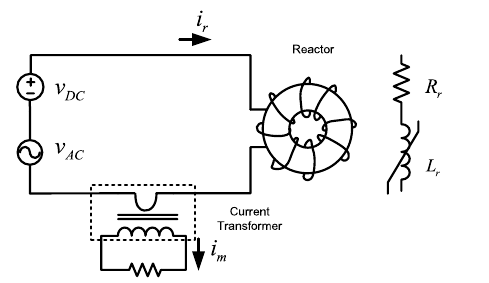
\includegraphics[width=.8\linewidth]{fig1.png}
    \end{figure}
\end{frame}

\begin{frame}
    \frametitle{Forma de onda esperada para uma carga não linear}

    \begin{figure}
        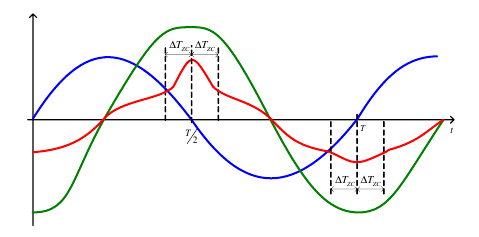
\includegraphics[width=.8\linewidth]{fig2.png}
    \end{figure}
    Onde:
    \begin{itemize}
        \item Onda azul, tensão aplicada no primário do reator
        \item Onda verde, fluxo magnético
        \item Onda vermelha, corrente de magnetização do transformador
    \end{itemize}
\end{frame}

\begin{frame}
    \frametitle{Detectando a componente DC}

    \begin{figure}
        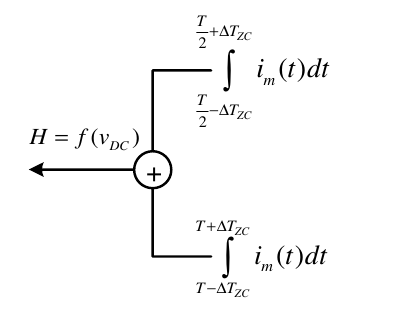
\includegraphics[width=.6\linewidth]{fig3.png}
    \end{figure}

    Onde: 
    \begin{itemize}
        \item $f(V_{DC})$ informa a amplitude e sinal da componente DC
    \end{itemize}

\end{frame}

\begin{frame}
    \frametitle{O esquemático completo}

    \begin{figure}
        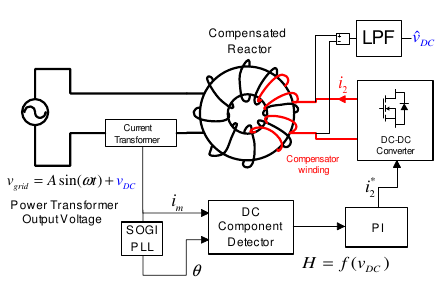
\includegraphics[width=.8\linewidth]{fig4.png}
    \end{figure}
\end{frame}

\begin{frame}
    \frametitle{Decompondo as componentes da senoide}

    \begin{figure}
        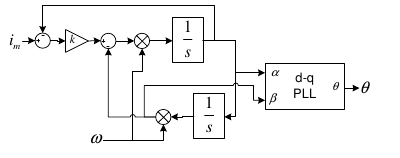
\includegraphics[width=.8\linewidth]{fig5.png}
    \end{figure}

    Sistema PLL-SOGI, tecnica usada para retirada de informações como tensão, corrente, frequencia... rejeitando as harmônicas menos significativas e aumentando a linearidade.
\end{frame}

\begin{frame}
    \frametitle{Resultados}

    Sistema em malha aberta, retirada de $i_m$

    \begin{figure}
        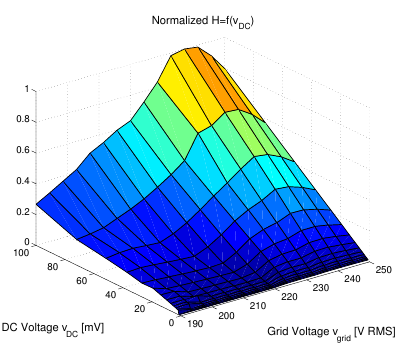
\includegraphics[width=.8\linewidth]{fig7.png}
    \end{figure}
\end{frame}


\begin{frame}
    \frametitle{Resultados}

    Sistema em malha fechada,

    \begin{figure}
        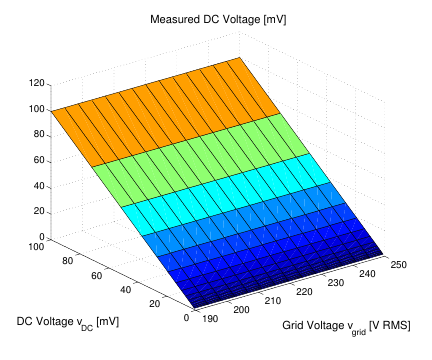
\includegraphics[width=.8\linewidth]{fig8.png}
    \end{figure}
\end{frame}


\begin{frame}
    \frametitle{Sistemas trifásicos}


    \begin{figure}
        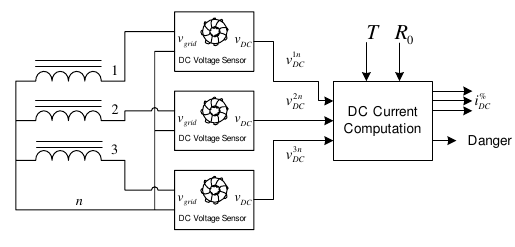
\includegraphics[width=.8\linewidth]{fig10.png}
    \end{figure}
\end{frame}

\begin{frame}
    \frametitle{Resultados práticos}
    
    Prototipo do reator,
    \begin{figure}
        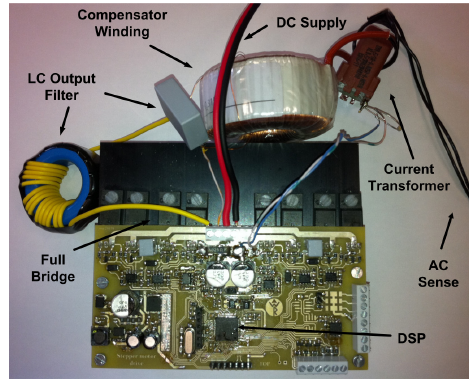
\includegraphics[width=.8\linewidth]{fig11.png}
    \end{figure}
\end{frame}

\begin{frame}
    \frametitle{Resultados práticos}

    Montagem completa,
    \begin{figure}
        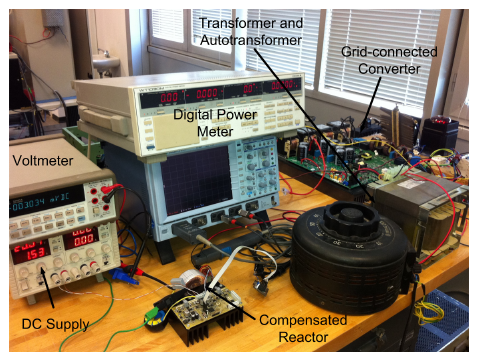
\includegraphics[width=.8\linewidth]{fig13.png}
    \end{figure}
\end{frame}

\begin{frame}
    \frametitle{Resultados práticos}

    Linearidade do sensor
    \begin{figure}
        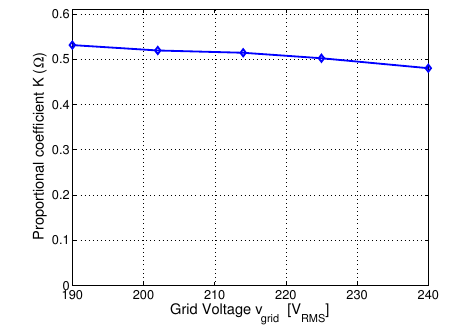
\includegraphics[width=.8\linewidth]{fig15.png}
    \end{figure}
\end{frame}

\begin{frame}
    \frametitle{Resultados práticos}

    Valor de H, corrente e compensação
    \begin{figure}
        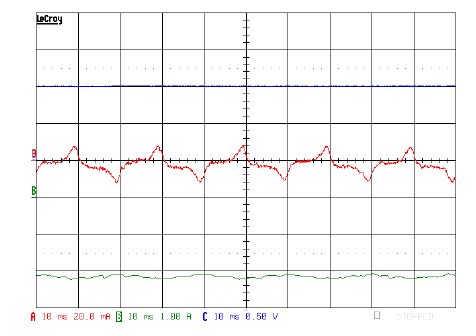
\includegraphics[width=.7\linewidth]{fig17.png}
    \end{figure}
    \begin{itemize} 
        \item onda azul, valor da componente DC
        \item onda vermelha, corrente de saturação
        \item onda verde, corrente de compensação $i_m$
    \end{itemize}
\end{frame}




\end{document}


